\chapter{Work Completed}\label{chapter:work}

%This should discuss what progress has been made on designing, implementing and evaluating the artifact. Care must be taken to ensure that any discussion of technical points are clearly explained, with diagrams being used where appropriate.
%In many cases, the evaluation proper will not yet have begun. However, it is important to demonstrate that sufficient thought has been given to the evaluation.

% Consideration of test generation techniques used
% Trade off => Performance vs accuracy?
% Needed to create test cases that adhered to the pre-conditon

An implementation of the tool has been created with generation of core data types. The tool has also been extended to use integer range analysis.

For a user to use the tool, a user must pass in a WYIL file and specify the test case generation technique to use, number of tests they wish to generate and ranges for generating integers.
% TODO ranges
Ranges are used to bound the integers generated so that ...

\section{Test Case Generation Techniques}

QuickCheck for Whiley currently employs two different techniques to generate test cases: random test-case and exhaustive test case generation.

\subsection{Random Test Case Generation}

A fixed number of tests determined by the user is randomly generated. Previous inputs are not considered which may lead to the same inputs being generated. 
% TODO refer Knuth Algorithm S
Algorithm ... was considered to generate unique inputs but has not been implemented yet.

\subsection{Exhaustive Test Case Generation}
A fixed number of tests determined by the user are exhaustively generated within a bounded range from the minimum bound to the maximum bound. All possible input combinations for a function are tested starting from the combination generated from the minimum bound.

\section{Data types generated}
Different generators are created for the different types defined in Whiley. 
Figure \ref{fig:qc-generators} illustrates the structure of the generators used.
Each generator generates a value. It also has a size for the number of input combinations and \texttt{resetCount()} and \texttt{exceedCount()} methods for monitoring input combinations generated for test-case generation.
 
\begin{figure}
	\caption{Class diagram of Generators in QuickCheck for Whiley}
	\label{fig:qc-generators}
	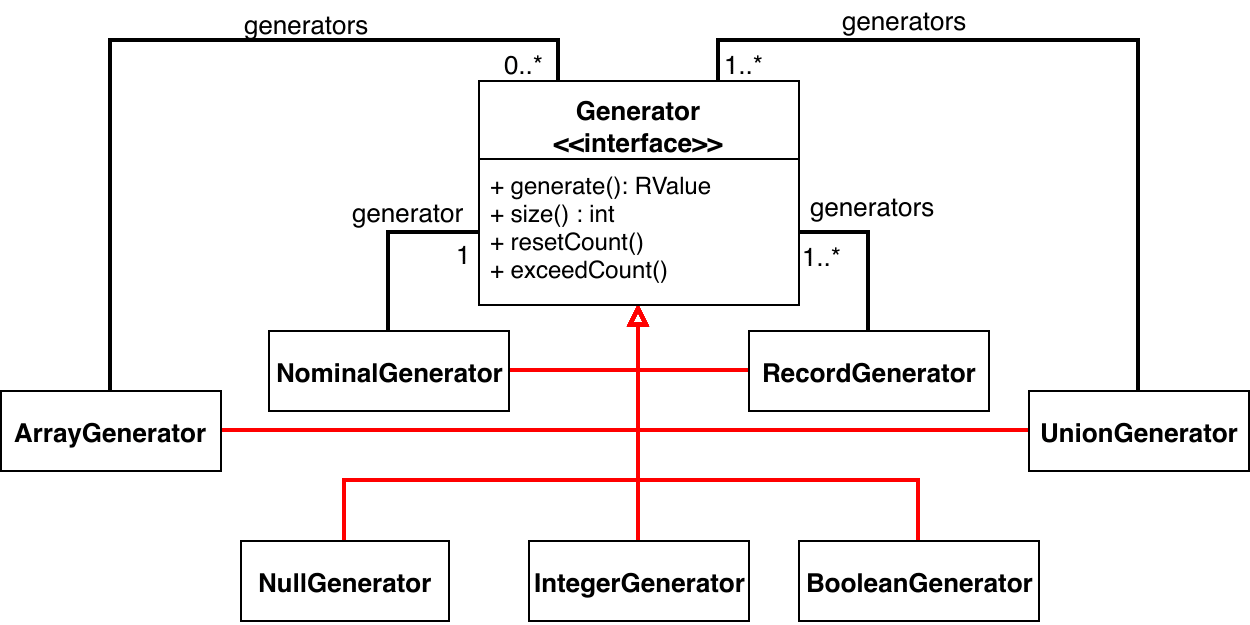
\includegraphics[width=\textwidth]{qc-generators}
	\centering
\end{figure}


% TODO add class diagram for generators

% TODO make a list of the types used

\begin{description}
	\item[Null] Generate a null value.
	\item[Boolean] Generates a boolean which is either true or false.
	\item[Integer] Generates an integer between a bounded range. This range may be modified based on constraints applied to the integer.
	\item[Array] Generates an array with a specific element type between a bounded size range.
	The size of arrays are currently limited to a maximum size of three elements due to the performance cost of generating larger arrays.
	\item[Nominal] A nominal represents a user-defined type by redefining a type with a different name \cite{WhileyLang}. Therefore, a generator for a nominal wraps a generator for a different type to generate a value. A nominal can also have a type constraint/invariant applied to it \cite{WhileyLang}.
	\item[Record] "A record type describes the set of all compound values made from one or more fields, each of which has a unique name and a corresponding type \cite{WhileyLang}." 
	A closed record is generated by generating values that correspond to each field. Generators corresponding to each field is required as each field may have different types. 
	% TODO Open records have not been implemented
	\item[Union] A union is made up of multiple types where the value can correspond to any one of the types declared. For example, the type \texttt{bool|int} can hold either a boolean or an integer value. 
	A union is generated by generating a value from one of the declared types. A generator corresponding to each type is required. 
	% TODO Talk about fairness in union generation
\end{description}

% Talk about generators here
% Class diagram of the ranges
% Talk about the different types



\section{Integer Range Analysis}

Integer range analysis is ... 
% Refer to paper 

\section{Evaluating the tool}
The tool has been evaluated by executing a variety of tests notably, the test suite for the Whiley Compiler.
%As a result, ... 
% Talk about how the tool is run
% Talk about evaluating the tool using the Whiley valid and invalid tests
% How to evaluate the tool